%%%%%%%%%%%%%%%%%%%%%%%%%%%%%%%%%%%%%%%%%
% Vertical Line Title Page 
% LaTeX Template
% Version 1.0 (27/12/12)
%
% This template has been downloaded from:
% http://www.LaTeXTemplates.com
%
% Original author:
% Peter Wilson (herries.press@earthlink.net)
%
% License:
% CC BY-NC-SA 3.0 (http://creativecommons.org/licenses/by-nc-sa/3.0/)
% 
% Instructions for using this template:
% This title page compiles as is. If you wish to include this title page in 
% another document, you will need to copy everything before 
% \begin{document} into the preamble of your document. The title page is
% then included using \titleGM within your document.
%
%%%%%%%%%%%%%%%%%%%%%%%%%%%%%%%%%%%%%%%%%

%----------------------------------------------------------------------------------------
%	PACKAGES AND OTHER DOCUMENT CONFIGURATIONS
%----------------------------------------------------------------------------------------

\documentclass{article} 
\usepackage{titlesec}
\usepackage[utf8]{inputenc}
\usepackage{tocloft}
\usepackage[margin=1in]{geometry}
\usepackage{graphicx}
\usepackage{enumitem}
\renewcommand{\cftsecleader}{\cftdotfill{\cftdotsep}}

\newcommand*{\plogo}{} % Generic publisher logo

\usepackage{float,array}
\usepackage{chngcntr}
\counterwithin{figure}{subsubsection}
\usepackage{booktabs} % To thicken table lines

%----------------------------------------------------------------------------------------
%	TITLE PAGE
%----------------------------------------------------------------------------------------

\newcommand*{\titleGM}{\begingroup % Create the command for including the title page in the document
\hbox{ % Horizontal box
\hspace*{0.2\textwidth} % Whitespace to the left of the title page
\rule{1pt}{\textheight} % Vertical line
\hspace*{0.05\textwidth} % Whitespace between the vertical line and title page text
\parbox[b]{0.75\textwidth}{ % Paragraph box which restricts text to less than the width of the page

{\noindent\Large\bfseries Software Design Document \\[0.5\baselineskip] for Smart Fridge Kitchen Assistant}\\[2\baselineskip] % Title
{\tiny \textit{Prepared by the Smart Fridge Team}}\\[4\baselineskip] % Tagline or further description
{\Large \textsc{joshua wilson\\sai sivva\\ahmed humayun\\shu yang\\zhen li}} % Author name

\vspace{0.5\textheight} % Whitespace between the title block and the publisher
{\noindent CSC 532: Software Engineering \plogo}\\[\baselineskip] % Publisher and logo
}}
\endgroup}

\setcounter{tocdepth}{2}
%----------------------------------------------------------------------------------------
%	BLANK DOCUMENT
%----------------------------------------------------------------------------------------
\titleformat{\subsubsection}[runin]
{\normalfont\normalsize\bfseries}{\thesubsubsection}{1em}{}
\begin{document}

\pagestyle{empty} % Removes page numbers

\titleGM % This command includes the title page
\tableofcontents
\vfill
\section*{Revision History}
{\ttfamily\begin{center}
		\begin{tabular*}{\textwidth}{ m{4em} m{5em} m{25em} m{4em}  }		
			\toprule			
			Rev.\# & Date & Nature of Revision & Version \\
			\bottomrule
			\toprule
			1 & 10.30.2016 & ORIGINAL VERSION & 1.0\\
			2 & 11.01.2016 & Added to  Profile and Item Classes & 1.0\\
			\hline		
		\end{tabular*}
	\end{center}
}
\pagebreak

\section{Introduction}

\subsection{Purpose}
The main purpose of the Software Design Document (SDD) is to provide information on the implementation of the Smart Fridge: Kitchen Assistant. The Smart Fridge: Kitchen Assistant is software developed to help individuals and families take care of their 

\subsection{Scope} The scope of this project is to refine the existing Smart Fridge Project. This includes creating a user interface for using for a touch screen platform, implementing a customizable nutrition plan for the user, broadening the project to include several inventories, and allowing for a bulk fridge update using information from receipts. Additionally, the product will allow for integration with the Pillar smart house project.

\section{Design Overview}

\subsection{Description of Problem} The existing Smart Fridge project does not have a feature to bulk update. Therefore, the user must manually input all foods into the fridge which is a tedious endeavor. Additionally, the current Smart Fridge project does not provide nutritional information or track the users consumption. Moreover, the exiting Smart Fridge project does determine waste or recommend a temperature for foods in the refrigerator. With these features, the user will be able to more easily use the Smart Fridge to help them live healthier and to help them reduce their environmental impact. 
\subsection{Technologies Used} This project uses Java EE to create a web-based application to be implemented in full screen on a 3rd generation Raspberry Pi. 
\subsection{System Features} 


	\subsubsection{Bulk Update, and Generalized Inventory}--This allows for the user to use electronic receipts to update many items into the fridge at once. Connecting with the Nutritionix API, the software will be able to provide nutritional information given Universal Product Codes (UPCs). 
				\begin{figure}[p]
					\centering
					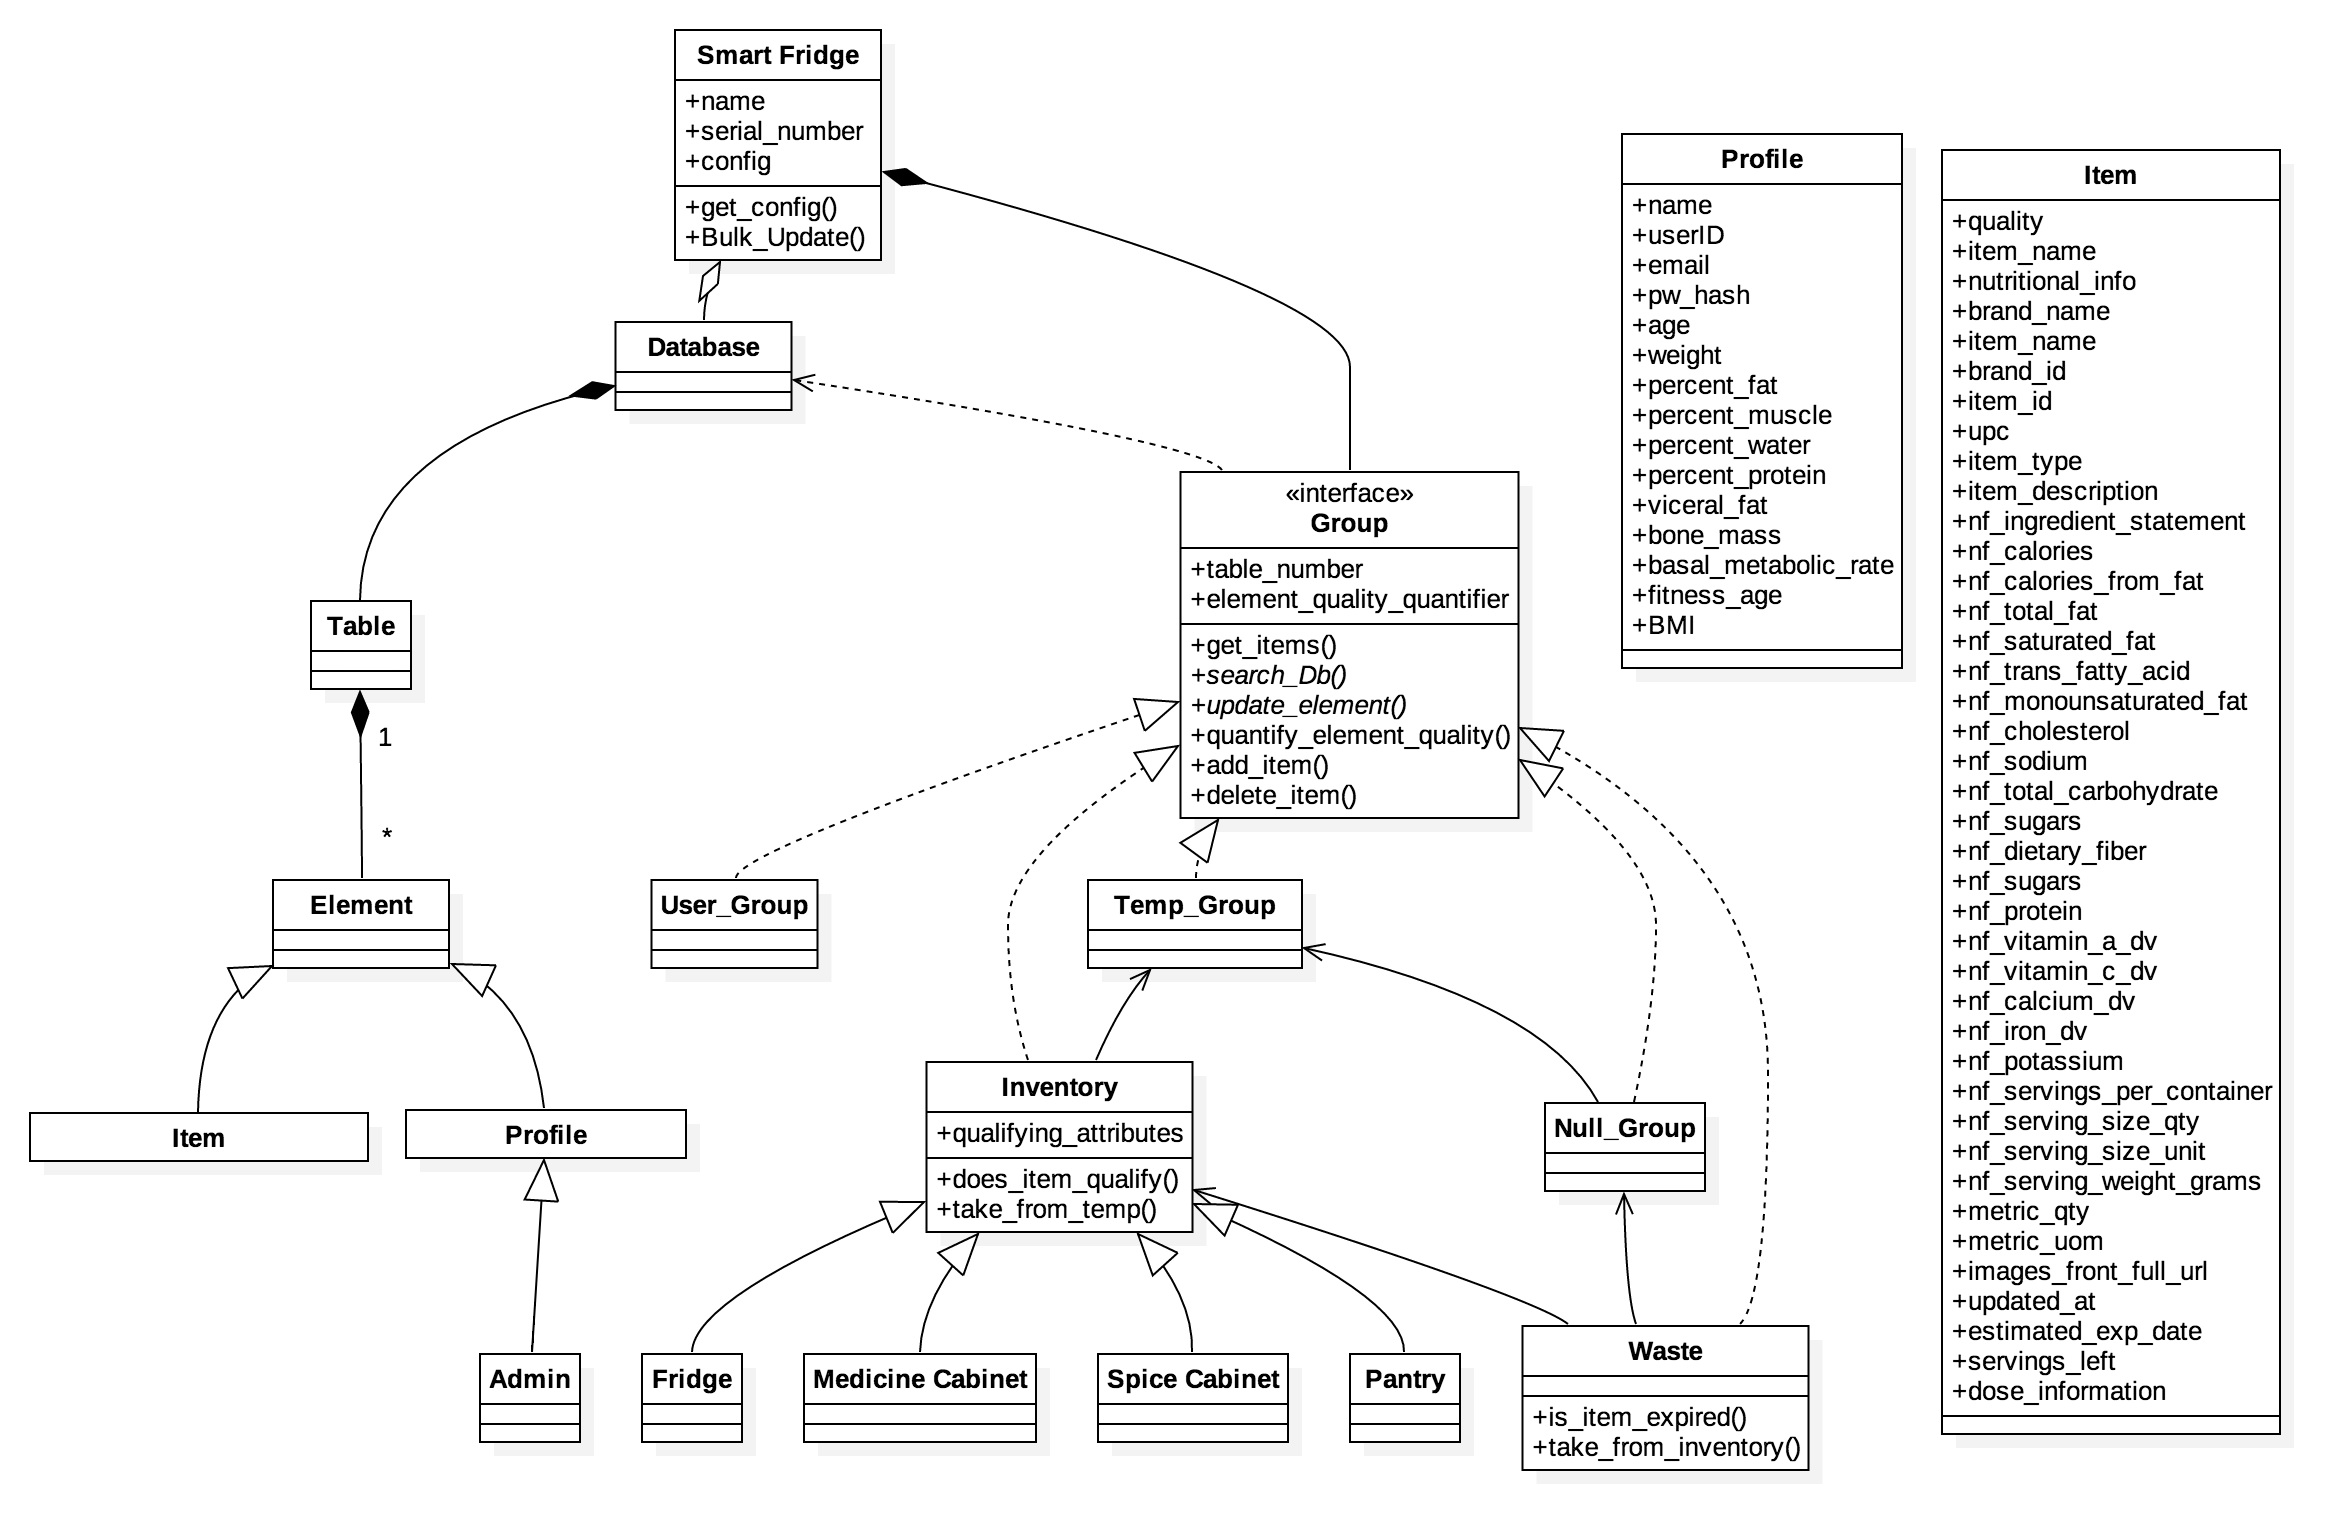
\includegraphics[width=\textwidth]{bulkupdate.png}
					\caption{Class Diagram: Bulk Update, and Generalized Inventory}
				\end{figure}
				\begin{figure}[p]
					\centering
					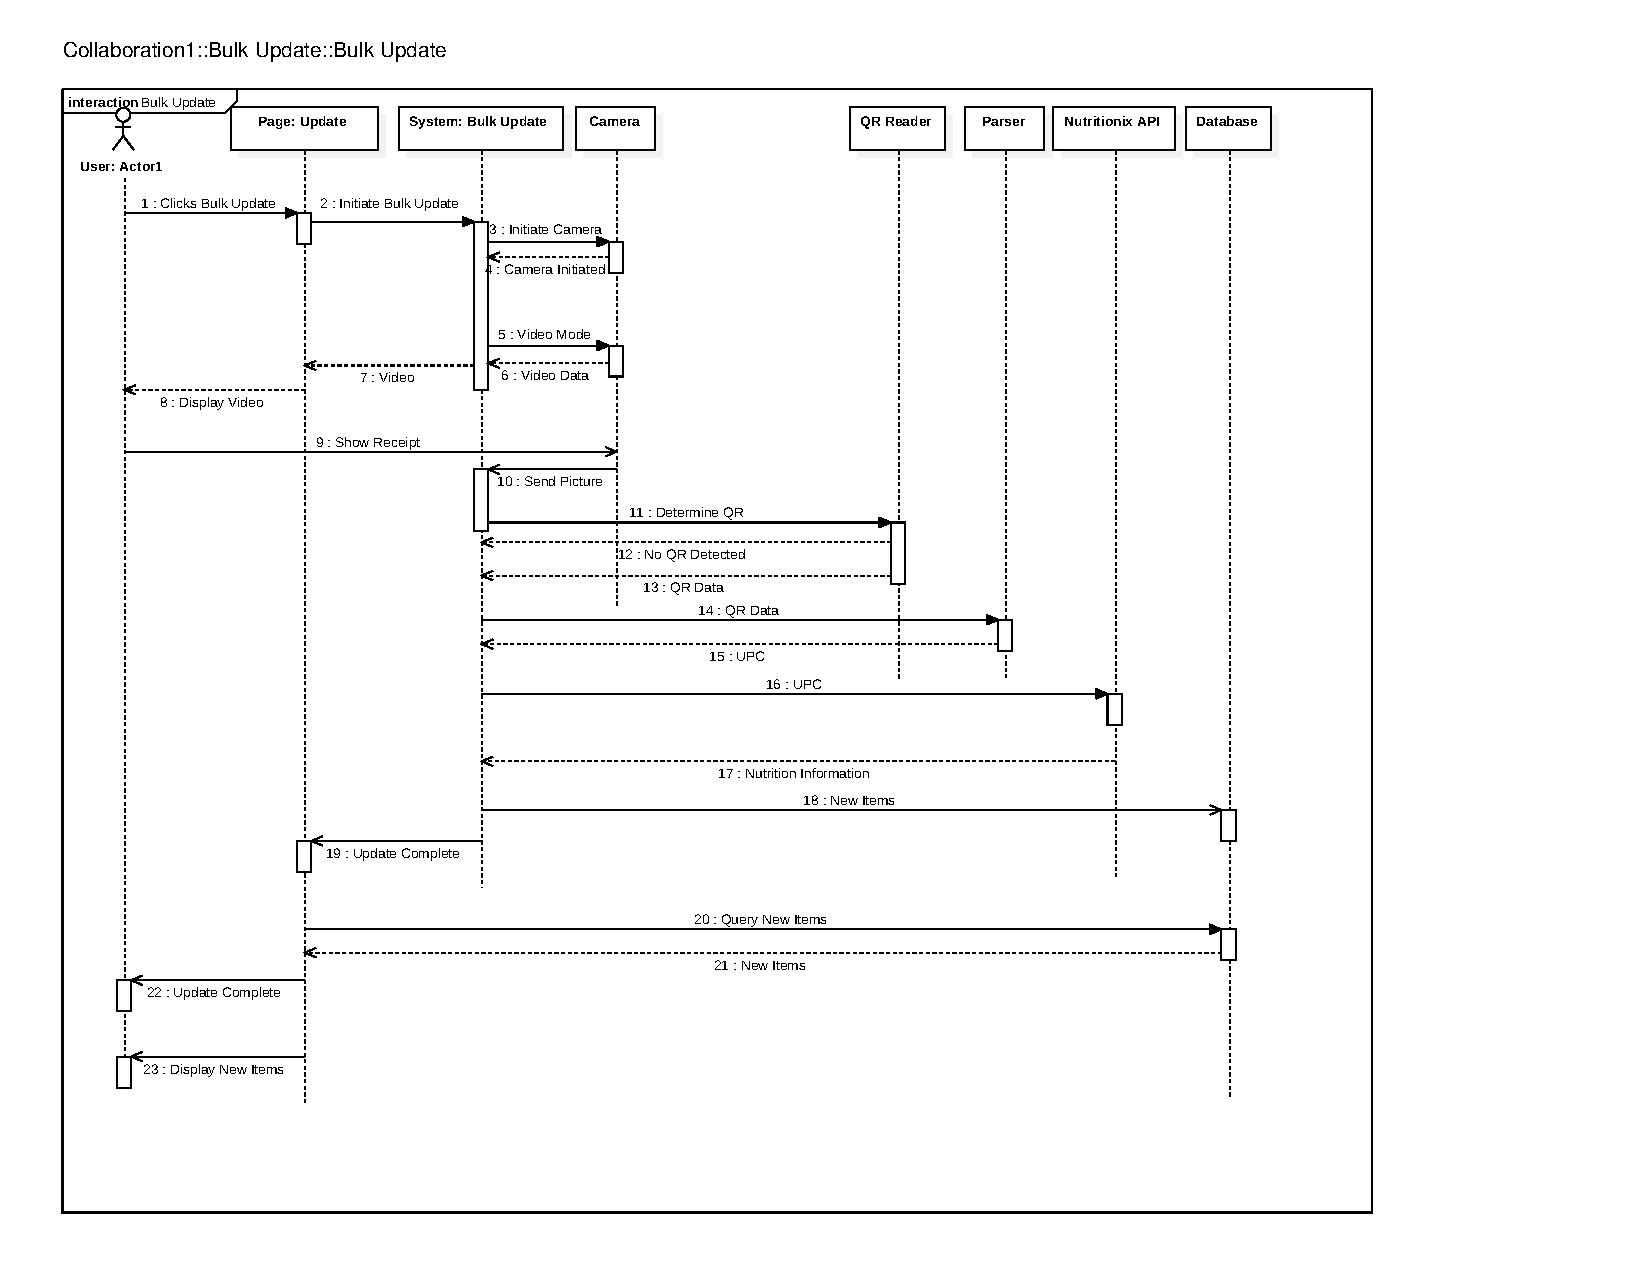
\includegraphics[width=\textwidth]{bulkupdate.pdf}
					\caption{Sequence Diagram: Bulk Update, and Generalized Inventory}
				\end{figure}
	\subsubsection{Nutritional Recommendation} The software keeps track of an individuals calorie intake and recommend meal plans based on the individuals input. 
	
			\begin{figure}[p]
				\centering
				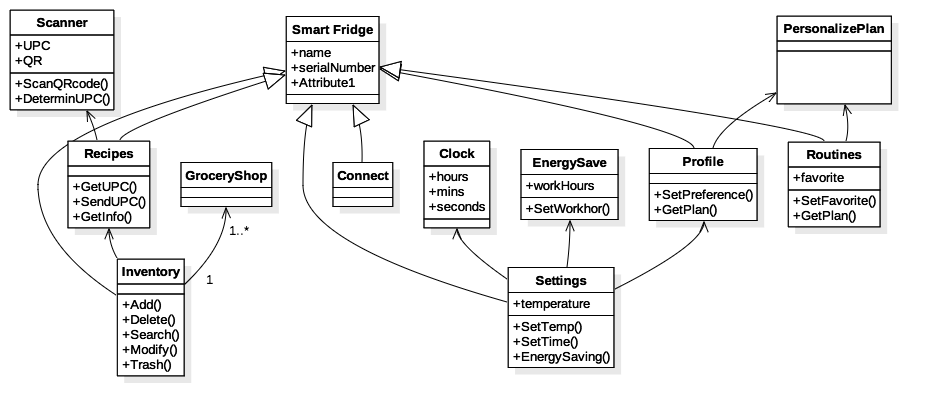
\includegraphics[width=\textwidth]{0ClassDiagram1_1.png}
				\caption{Class Diagram: Nutritional Recommendation}
			\end{figure}
			\begin{figure}[p]
				\centering
				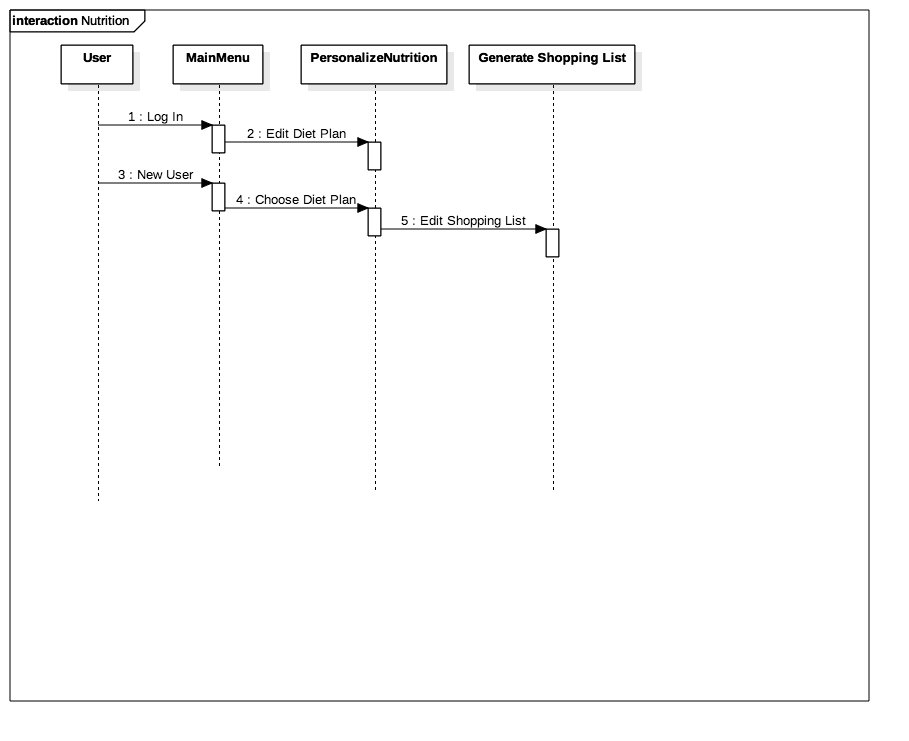
\includegraphics[width=\textwidth]{0SequenceDiagram_Nutrition.png}
				\caption{Sequence Diagram: Nutritional Recommendation}
			\end{figure}
			 
	\subsubsection{Waste Approximation \& Energy Saving} The system tracks waste, and provides a waste estimation. Additionally, the system recommends a temperature at which to keep the refrigerator based on the contents. 
	
		\begin{figure}[p]
			\centering
			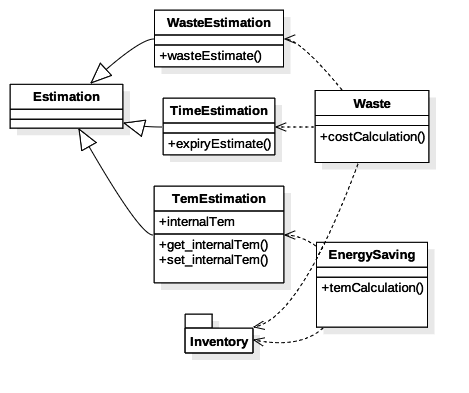
\includegraphics[width=\textwidth]{ClassDiag-Eco.png}
			\caption{Class Diagram: Waste Approximation \& Energy Saving}
		\end{figure}
		\begin{figure}[p]
			\centering
			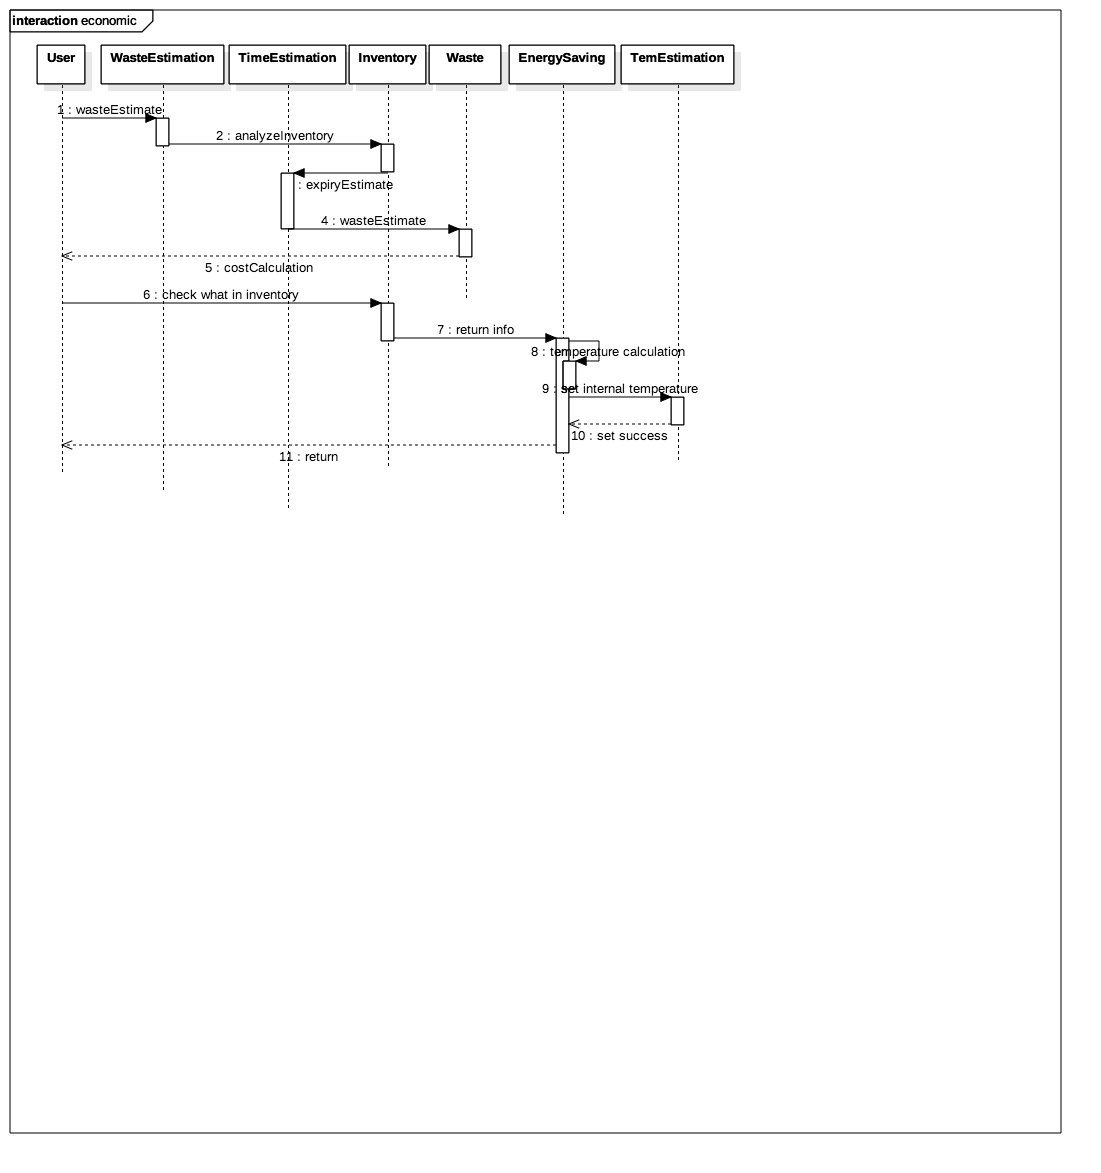
\includegraphics[width=\textwidth]{eco_sequence_conomic_3.png}
			\caption{Sequence Diagram: Waste Approximation \& Energy Saving}
		\end{figure}






\end{document}